\documentclass[submission,copyright,creativecommons]{eptcs}
\providecommand{\event}{SOS 2007} % Name of the event you are submitting to
\usepackage{breakurl}             % Not needed if you use pdflatex only.

\def\focalize{FoCaLiZe \mbox{}}


\usepackage{graphicx}


\title{Teaching Formal Methods with Discrete Mathematics  {\it versus} 
  Teaching Discrete Mathematics with Formal Methods}

\author{Mathieu Jaume
\institute{Sorbonne Universit\'es, UPMC Univ. Paris 06 \\ UMR 7606 ,
  LIP6 \\  F-75005, Paris, France}
\email{Mathieu.Jaume@lip6.fr}
\and Th\'eo Laurent
\institute{Sorbonne Universit\'es, UPMC Univ. Paris 06 \\ F-75005, Paris, France}
\email{Theo.Laurent@etu.upmc.fr}
}
\def\titlerunning{Teaching: Formal Methods {\it versus} Discrete Mathematics}
\def\authorrunning{M. Jaume, T. Laurent}
\begin{document}
\maketitle

\begin{abstract}
Despite significant advancement in the conception of (formal) integrated
development environments,
applying formal methods in software industry is still perceived as
a difficult task. To make the task easier, providing tools that help
during the development cycle is essential but we think that
education of computer scientist and software engineers is also an
important challenge to take up. Indeed, we believe that applying formal methods 
is perceived as a difficult task because
formal methods courses 
do not appear sufficiently early in compter science curricula. In this
paper, we claim that teaching formal methods could be done at the
undergraduate level by mixing formal methods and discrete mathematics
courses and we illustrate such an approach with a small development within FoCaLiZe.
We also believe that this could considerably benefit the learning of
discrete mathematics. 
\end{abstract}

\section{Introduction}


Nowadays,
critical systems are evaluated according to some standards like the
Common Criteria~\cite{CC2} or
according to standards dedicated
to particular domains.
These standards often
require the use of formal methods in order to ensure some safety and
security properties needed of the systems in question.
Indeed, for large developments ad hoc approaches have proven inadequate to assure
that the delivered software satisfies some safety and security
requirements. In fact,
the lack of formalisation often leads to produce systems whose
behaviors are not fully and precisely understood.
Formal methods aims at helping to build systems with high
safety and security assurances,  
by
providing formal integrated development environments (F-IDE) that help to specify, to document,
to implement, to test, to prove or to analyse critical systems.
Of course, such environments often ease
(and partially automate)
the application of formal methods during the development cycle, but
developing (and evaluating) critical systems is a
difficult task that still
requires advanced technical knowledge and large amounts of time.
Hence, formal methods
are still not sufficiently used in industrial software
development. 

Developing F-IDE that ease the application of
formal methods remains a challenging issue but we believe that education is
also one challenge to take up to promote the use of formal methods in
the software creation process:
the formal methods community has not enough focused its
attention to the education of computer scientist and software
engineers, especially at the undergraduate level.
Indeed, many computer science curricula
do not contain formal courses, or such 
materiel is not introduced sufficiently early. 
Of course, almost all computer science curricula include discrete mathematics courses but
often in isolation from computer science, leaving students
understanding little about why (and how) mathematics applies to computer science
and {\it vice versa}. 
Teaching discrete mathematics is still often done in the traditional
way, using pen and paper.
Therefore, many computer science students are rather
``math-averse'', perceive mathematics as a difficult discipline and
don't  understand the relevance of mathematics in their curricula.

Therefore, sometimes, discrete mathematics courses 
use functional programming languages (such as ML, OCAML, HASKELL, etc.)  to reinforce mathematical concepts.
There exists now some discrete mathematics
texbooks~\cite{Doets04,books/daglib/0007497,bookvandrunen} based on
such an approach whose
benefits are discussed 
in~\cite{DBLP:conf/sigcse/Wainwright92,oai:CiteSeerXPSU:10.1.1.19.3780,darosa02,Henderson02,DBLP:conf/oopsla/VanDrunen11}.
In~\cite{DBLP:conf/oopsla/VanDrunen11}, the author goes further 
by considering that computing is also a vital topic for
contemporary mathematics students and that they will 
need some level of competency in programming at some point in their
professional practice. Hence, the author claims
that the
integrated work of mathematics and
computer science educators could considerably benefit the learning of
both subjects: putting functional programming and
discrete mathematics in the same course, provides a useful service for
both computer science and mathematics students.
Functional programming languages are high-level languages
and thus are well suited to teach discrete
mathematics. Indeed, 
they permit to implement mathematical concepts without considering low level
issues such as data representation and memory allocation. Hence, 
mathematical notions can be ``easily'' introduced together with their 
implementations (that remain very
close to the concepts that get implemented) and can be experimented
by students.
Dealing with a programming language to teach discrete mathematics can
also be useful to illustrate how some specification and
reasoning techniques (logic, induction) apply to
computer science when proving that a program meets its specification. The goal in this part of material is to show
how to ensure a high value on the correct operation of computing which
is one of the main purposes of formal methods. However, at the
undergraduate level, programming languages are only used as a formalism to manipulate
the computational part of mathematical objects but not to express specifications or to
implement proofs. 
This leads to view formal methods as {\it a posteriori}  methods in the
programming tasks. In this paper, we claim that formal methods also provide 
an {\it a priori} help during the conception of software
that can be
taught in discrete mathematics courses: 
designing the architecture of a software and specifying a hierarchy of
mathematical discrete structures are very similar tasks. 

Even if proof assistants seem now to be mature enough to be adaped to the education,
at undergraduate level, formal reasoning is seldom introduced and
mostly appears in ``pure'' logic courses. For example, 
in~ \cite{hendriks-adn10}, the design of a web interface for Coq used to teach
logic to undergraduate students is presented. 
In the context of computer science, formal reasoning is generally introduced at
a more advanced stage. This can be done by implementing some automated
theorem proving techniques (like in \cite{Harrison09}) or by using
proof assistants such as Coq or Isabelle.
In this case, F-IDE and theorem proving are not objects of the study but are
rather considered 
as a framework for teaching something else. Hopefully, using a language
as a vehicle for reinforcing concepts inevitably leads to learn some
methodological  and practical knowledges
about it.
For example, \cite{NKtoappear} is a semantics
textbook (to master students)  which is entirely based on the proof assistant
Isabelle.
The main benefit of using a proof assistant in
the teaching of semantics is that allows students to experiment their
specifications and to make
proofs by using a
computer program, which guides them through the development of
a completely correct proof and gives them immediate feedback.
This avoids 
students to produce ``almost-but-not-completely-right proofs'' (as
called by Pierce in \cite{DBLP:conf/icfp/Pierce09}) or even worse ``LSD trip proofs''
(as called by Nipkow in~\cite{Nipkow-VMCAI12}).
%The benefits of using proof assistants in
%the teaching of mathematics is also discussed
%in~\cite{narboux:inria-00495952}.


As we said, we think that teaching formal methods to beginning
students
is essential to disseminate their use in the software industry. However, at
the undergraduate level, no prerequesites on computer science can be
assumed and we can only suppose some very basic knowledges in
mathematics that are also considered as prerequisites in the first
courses of discrete mathematics. Hence, we believe that using a F-IDE
could be helpful to teach both computer science and discrete
mathematics in a mixed course and this paper aims at presenting a
small development illustrating the benefits of such an approach to
both disciplines. In this context, the F-IDE used as a teaching tool
must be suitable to express specifications
(i.e. properties), to write programs (i.e. definitions) and to make
proofs. One of the main issues is concerned with proofs. Within most theorem
provers, proofs are sequences of commands (belonging to a scripting
language)  that are hard to read for the
human and that do not clearly reflect the (tree) structure of 
proofs. Furthermore, the proof language used must be abstract enough
to avoid to teach the fine structure of logic (the inference rules)
and to automate the ``trivial'' steps of proofs by allowing students
to only express what intermediate steps
might help the proof assistant to complete proofs.
For these reasons, we think that  the \focalize\cite{foc03} F-IDE is a good candidate
to teach both computer sciences and discrete mathematics at the
undergraduate level.
Indeed, \focalize is an object-oriented programming environment that
combines specifications, programs and proofs in the same language. This
features can be used to
formally express specifications and to develop
the design and implementation of software as well as some hierarchy of
mathematical structures,
while proving that implementations meet their specifications or design
requirements.  
The object-oriented
features of this language enable the development of an implementation
by iterative refinement of its specification. Moreover, \focalize
provides several automatic tools to ease the generation of programs
from specifications, the generation of
proofs by the Zenon ``automatic'' theorem prover~\cite{conf/lpar/BonichonDD07}, the generation of
documentation, and the production of
test suites~\cite{DBLP:conf/icsoft/CarlierDG10}.
Moreover, many software
components implemented within \focalize can be directly built by
inheritance and parameterization from already defined components.
Hence, such developments can easily be reused in different contexts.







\section{\focalize}




\focalize\cite{foc03} is a F-IDE
which was conceived from the
beginning to help build systems with high
safety and security assurances. \focalize includes
a language based on firm theoretical
results~\cite{PrevostoJAR02}, with a clear semantics and provides an efficient
implementation -- {\it via} translation to OCaml~\cite{ocamldocu}.  It has
functional and object-oriented features and
provides means for the programmers to write formal proofs
of their
code
in a more or less detailed way
within a declarative proof language based on the Zenon automatic
theorem prover~\cite{conf/lpar/BonichonDD07}.
Zenon eases the task of writing formal proofs and
translates them into Coq~\cite{coq84} for high-assurance checking.
\focalize also provides powerful features (such as
inheritance, parameterization and late-binding) that enable
a stepwise refinement methodology to go from specification all the way
down to executable code.
Thus, \focalize unifies within the same language the formal modeling
work, the development of the code, and the certification proofs.
Very important is the possibility in \focalize to have
specifications, implementations and proofs \emph{within the same
language}, since it
eliminates the errors introduced between layers, at each switch
between languages, during the development cycle.
Other frameworks like Atelier B~\cite{Abrial96a} also aims to implement
tools for making formal development a reality. \focalize doesn't follow
the same path, trying to keep the means of expression close to what
engineers usually know: a programming language.
Moreover, instead of having its own system for proofs validation,
\focalize makes use of external tools, leaving the task of handling
proof automation and verification outside its scope and reaping
the benefits of research performed by others in these specific domains.
Of course, nowadays, proof assistants also provide some features for
structuring code (module systems, type classes, etc), but most of them
still cannot be used
to obtain efficient programs. 
Compilation of \focalize developments leads to efficient OCaml programs
(which are not obtained by extracting computational contents of
proofs). It is this focus on efficiency that makes \focalize a real programming
language. To our knowledge, only the Agda~\cite{conf/tphol/BoveDN09}
programming language, based on dependent types and compiling {\it via}
Haskell, has a comparable mix of features.
Note that the \focalize language is also based on a
dependent type language, but with some restrictions on dependencies.
%:
%for instance, a function
%cannot depend on a proof.  By allowing such dependencies, we might get
%a better treatment of partial functions, but function redefinition
%would get trickier to handle because of logical clashes.
%In practice, this seems
%too difficult and we have rejected this possibility.










\subsection{Species}


In \focalize, the primitive entity of a development is the \emph{species}.
Species are the nodes of the
hierarchy of structures that makes up a development.
A species can be seen as a set of methods grouping ``things'' related
to the same concept. As in most modular design systems
(i.e. object-oriented, abstract data types, etc.) the idea is
to group a data structure with the operations on the data structure, the
specification of these operations (in the form of properties), the
representation requirements, and the proofs of the properties.
Each method is identified by
its name and can be either declared 
(primitive constants, operations and properties)
or defined (implementation of operations, definition of properties and proofs of theorem).
Moreover, we can distinguish three kinds of ``methods'': the carrier type, the
programming methods and the logical methods (all the fields of our
objects are called methods, be they types, data or code).

\paragraph{Carrier type}
The carrier, or representation type, is the concrete representation of
the elements of the set underlying the structure defined
by the species. 
The carrier is represented by the keyword {\small \tt Self} inside
the species and outside, by the name of the species itself, so that we
identify the
set with the structure, as usual in mathematics.
Each species must have one unique carrier, but like all the other methods, it
can be either declared or defined. A declared carrier is simply an abstract 
data type, while a defined one is a binding to a concrete type.

\paragraph{Programming methods}
These methods represent the constants and the operators of the structure.
Declared methods are introduced by the keyword
{\small \tt signature}, defined methods are introduced by {\small \tt let} and recursive
definitions must be explicitely flagged with the keyword {\small \tt rec}. The
language used for the definitions is similar to the functional core of 
OCaml~\cite{ocamldocu} (let-binding, pattern matching, conditional,
higher order functions, etc),
with the addition of a construction to call a method from a given
structure. More precisely, the main syntactic constructions of the
language are the following:
\begin{itemize}
\item abstraction with respect to a variable: {\small \tt fun x -> ...}
\item application of a function: {\small  \tt f(x)}
\item call of a method {\small \tt m} from a structure {\small \tt c}: 
{\small \tt c!m}
\item call of a method {\small \tt m} of the structure we are currently building:
{\small \tt Self!m} or just {\small \tt m}
\end{itemize}

\paragraph{Logical methods}
These methods represent the properties of
programming methods. In this context, the declaration of a logical method 
is simply the statement of a property, while the definition is a proof of
this statement. In the first case, we speak of {properties} ({\small
  \tt property}) that are still
to be proved later in the development, while in the second case we speak of
{theorems} ({\small \tt theorem}). 
The language also allows logical definitions ({\small \tt logical
  let}) to bind names to logical statements.
The language used for the statements is composed of the basic logical
connectors {\small \tt and}, {\small \tt or}, {\small \tt ->}, {\small \tt <->}, {\small \tt not}, 
and universal ({\small \tt all})
and existential ({\small \tt ex}) quantification over a \focalize type.
\focalize allows declarative proof descriptions inspired by Lamport's
work~\cite{Lamport95,chaudhuri:proof}. A proof is a tree where the programmer
introduces names ({\small \tt assume}) and hypotheses ({\small \tt hypothesis}), gives a statement to
prove ({\small \tt prove}) and then provides justification for the
statement. This justification can be: (1) a ``{\small \tt conclude}'' clause for
fully automatic proof; (2) a ``{\small \tt by}'' clause with a list of
definitions, properties, hypotheses, previous theorems, and previous
steps (subject to some scoping conditions) for use by the automatic
prover; (3) a sequence of proofs (with their own assumptions,
statements, and proofs) whose statements will be used by the automatic
prover to prove the current statement.
Hence, each step of a proof is independent of the others and can be
reused in a similar context (this eases the maintenance of proofs and
allows, for example, using exactly the same proof for a statement based on an
hypothesis $A$ and for the same statement based on a stronger
hypothesis $B$, provided the automatic prover can make the inference
from $B$ to $A$).



\subsection{Combining species}


\begin{figure}
  \begin{center}
    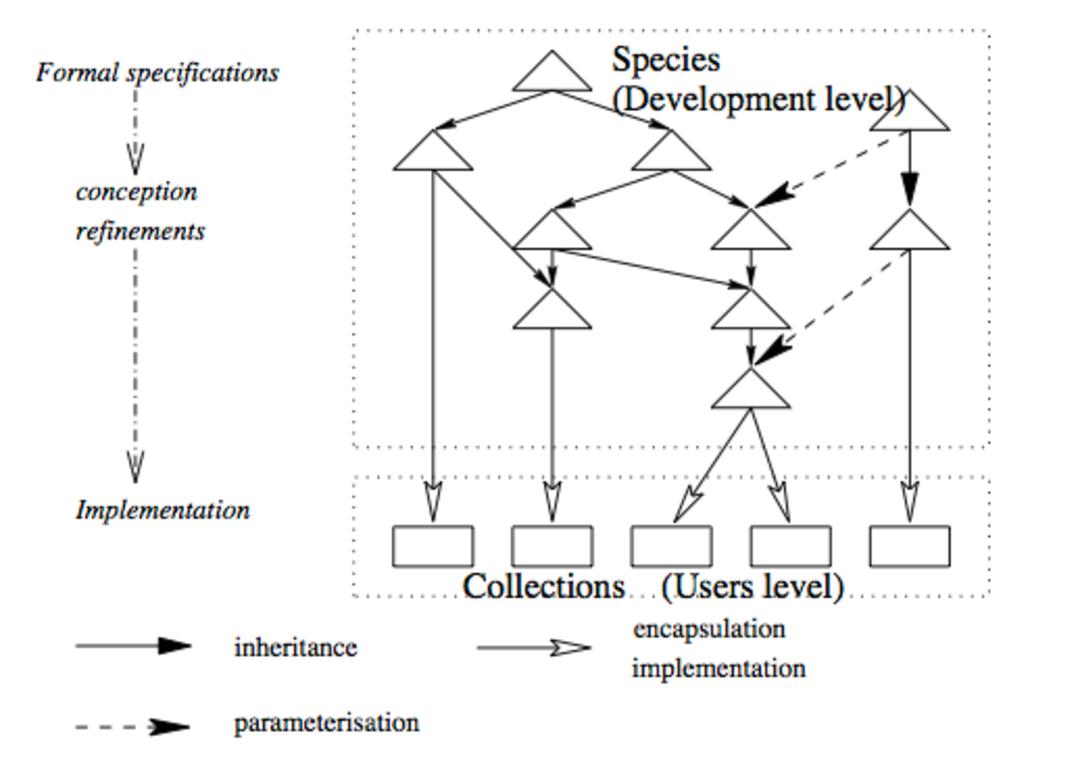
\includegraphics[width=9cm]{GFocal.pdf}
    \caption{\focalize}
    \label{fig:focal}
  \end{center}
\end{figure}

The main (object-oriented) features of \focalize are illustrated in
Figure~\ref{fig:focal}: a \focalize development is organized as a
hierarchy which may have several roots.
The upper levels of the hierarchy are built during the specification
stage while the lower ones correspond to implementations.

\paragraph{Inheritance}
Using inheritance in \focalize, one can
enrich a species with additional operations (methods) and
redefine some methods of the parent species, but one can also get
closer to a runnable implementation by providing explicit definitions to methods
that were only declared in the parent.
Note that the inheritance framework requires to perform static analysis in order
to check coherence properties (inheritance lookup, resolution of 
multiple-inheritance conflicts, dependency analysis, type-checking,
etc).
In \focalize, classical object-oriented features have been restricted
in order to
avoid unsound constructions that can lead to inconsistencies when used
carelessly.
A species can
inherit the declarations and definitions of one or several already
defined species and is
free to define or
redefine any inherited method as long as such (re)definition does not
change the type of the method.

\paragraph{Collections}

A collection is built upon a completely defined species. This means
that every method must be defined. In other words, in a collection, every 
operation has an implementation, and every theorem is formally proved.
In addition, a collection is ``frozen'': it cannot be used as a parent
of a species in the inheritance graph. Moreover, to ensure modularity
and abstraction, the carrier of a collection is hidden: seen from the
outside, it becomes an abstract type. This means
that any software component dealing with a collection will only be
able to manipulate it through the operations it
provides (i.e. its methods). This point is especially important since
it prevents other
software components from breaking representation invariants required by the
internals of the collection.

\paragraph{Parameterization}

Besides inheritance, another important feature of \focalize is the ability to
parameterize a species by generic collections instanciating a species. Such a
mechanism allows to use a species, not to embed its methods, but rather to
use it as an ``ingredient'' to build a new structure by calling its methods
explicitly.




\section{The example of binary relations}


conclusion : first lesson on relations and functions 1) maths 2)
formal methods 3) important notion of function in maths and computer science


\subsection{Definitions as Properties}

\subsubsection{Building formal specifications {\it versus} Understanding
  mathematical definitions as properties}

from absrtact binary relation to bijections

(multi)-heritage, parameterization


Ex: We define $k$ as an object such that $P(k)$.

\subsubsection{Formal reasoning on specifications {\it versus} Deducing
  properties from properties}

Ex: An object such that $P_1, \cdots, P_n$ is such that $P$.

composition de relation + quelles proprietes  ? 

preuve sur des specs

\subsection{Definitions as Computations}

\subsubsection{Programs {\it versus} Constructive definitions}

Ex: We define $k$ as obtained by $f(p)$

\subsubsection{Certified programming {\it versus} Deducing properties
  over computations}

implantation + preuves sur des implantations

Ex: $f(p)$ is such that ...

rajouter la species avec la fonction en param et qui definit la
relation avec les props. (cf LTS)


\section{Conclusion}

Many teaching experiences have been done by using F-IDE at master
level for computer science students and benefits of such approaches
are nowadays well recognised. For example, we have already
used~\cite{Coq-Ens} \focalize (together with Coq) to teach semantics of
object-oriented features of a programming languages. 
In this paper, we consider \focalize as a teaching tool at the
undergraduate level and illustrate such an approach by developping
a lesson of
discrete mathematics.
In addition to pedagogical benefits, 
we believe that teaching formal methods as earlier as possible leads to
raise the level of mathematical rigor for computer science so as to
ensure they are perceived as valid professional disciplines by
students. 
Formal methods will be of
increasing value in computer and software engineering (especially for 
safety-critical, security-sensitive, and embedded systems)
and we think that education is one challenge to take up 
in order to promote the dissemination of formal methods in software industry.



\focalize is a good candidate to mix both formal
methods and discrete mathematics courses. Indeed,  \focalize provides
a formal integrated development environment simple enough to be 
usable by most students at university (even if they are not fully
acquainted with theoretical concepts such as 
higher-order logics), in particular by making development
of correct proofs as easy as possible and as readable  as possible.
Moreover, \focalize leads to stress the process of
abstraction through the construction, step by step, of problem
solutions from their specifications. This can be helpful
to improve the learning process of discrete mathematics but also to
show to students that
computer
science involves a lot of mathematical activities and {\it vice versa}.


\focalize includes a
computer algebra library, mostly developed by
R.~Rioboo~\cite{calc01,DBLP:journals/amai/Rioboo09}, which
implements mathematical structures up to multivariate 
polynomial rings and includes complex algorithms
with
performance comparable to the best computer algebra systems in
existence.
Hence, as future works, we believe that \focalize could be used 
to develop a discrete
mathematics course.

% (including 
%symbolic logic and proofs, induction and recursion, set theory, functions and
%relations on sets, graph theory and languages and automata).








\paragraph{Acknowledgments}
The authors would like to thank B\'eatrice B\'erard, Damien Doligez, Th\'er\`ese Hardin,
Fran\c{c}ois Pessaux,  and Renaud Rioboo for enlightening discussions
about teaching formal methods and discrete mathematics.



%\nocite{*}
\bibliographystyle{eptcs}
\bibliography{fbibli}
\end{document}



Using these tools together
with an adequate methodology of development (as the one introduced
in~\cite{DBLP:journals/entcs/AyraultHP09}) also makes the developments
easier to formally evaluate  according to the aforementioned standards.
In the domains of safety and security, two main developments have been already
done within \focalize: a full formalization of airport security
regulations~\cite{DelahayeED06}, and 
the implementation of
a generic voter~\cite{DBLP:conf/tap/AyraultHP09}, which is a central
equipment of all
fault tolerant architectures, widely used for safety related systems.


Aids to
precision in each phase of software development 

Formal methods (FMs) are intended to provide the means for greater precision in
both thinking and documenting the preliminary stage of the software creation
process.

providing notations and tools that are readily
understood and used by practitioners,



educational tools used for conveying these concepts to students.



... is not very popular with students ... they feel SML is more linked
with mathematics than computer science


Hence, the main originality of \focalize is to provide an
object-oriented programming language that allows mixing
specifications, programs and
proofs.


Math majors will spend most of their time as undergraduates proving
things, and computer science majors will do a lot of programming; yet
they both need to do a little of the other. The fact is,
robust programs and correct proofs have a lot to do with each other,
not the least of which is that they both require clear, logical
thinking. We will see how proof techniques will allow us to check that
an algorithm is correct, and that proofs can prompt
algorithms. Moreover, the programming component motivates the
proof-based discrete math for the computer science majors and keeps it
relevant; the proof component should lighten the unfamiliarity that
math majors often experience in a programming course.


they lack the information what is
being proved at each point, and they lack structure. Proof language
close to the informal language of mathematics ... teach proofs, not
logic (fine structure of logic is studied) ... what intermediate step
might help the proof assistant


The software industry has a long-standing and well-earned reputation for
failing to deliver on its promises and it is clear that still nowadays, the
success of software projects with the current technologies cannot be assured.
For large complex projects ad hoc approaches have proven inadequate to assure
the correct behavior of the delivered software. The lack of formalization in
key places makes software engineering overly sensitive to the weaknesses that
are inevitable in the complex activities behind software creation. 

Formal methods (FMs) are intended to provide the means for greater precision in
both thinking and documenting the preliminary stage of the software creation
process. When done well, this can aid all aspects of software creation: user
requirement formulation, implementation, verification/testing, and the creation
of documentation. However, the maturing of formal techniques into real-life
software engineering involves providing notations and tools that are readily
understood and used by practitioners, and the integration of such tools with
activities that are far from the unrealistic assumptions that characterized
some earlier research in formal methods.

After decades of research, and despite significant advancement, formal methods
are still not widely used in industrial software development. This may be due
to the fact that the formal methods community has not enough focused its
attention to software engineering needs, and its specific role in the software
process. At the same time, from a software engineering perspective, there could
be a number of fundamental principles that might help to guide the design of
formal methods in order to make them more easily applicable in the development
of software applications.

The main goal of the workshop is to foster integration between the formal
methods and the software engineering communities with the purpose to examine
the link between the two more carefully than is currently the case.

Despite computer science and mathematics being kindred fields,
computer science major populations include many math-averse
students. Many are frustrated at the math requirements of the program
and are slow to un-
derstand the relevance. The situation is more likely to be aggravated than remedied when the discrete math course is taught by the mathematics department.
...
Com- puting is a vital topic for contemporary math majors. Many will
need some level of competency in programming at some point in their
studies, whether in professional practice as ac- tuaries, to introduce
algorithmic topics as high school math teachers, or in research as
graduate students. 
Unfortunately, many math majors find pro- gramming to be foreign and become frustrated when they do not see any immediate relevance for their mathematical stud- ies. Their frustration is especially understandable if they are dropped into a Java programming course that was not de- signed for their needs.
+
book \cite{bookvandrunen}
Discrete mathematics topics include symbolic logic and proofs, including proof by induction; number theory; set theory; functions and relations on sets; graph theory; algorithms, their analysis, and their correctness; matrices; sequences and recurrence relations; counting and combinatorics; discrete probability; and languages and automata. All of these would be appropriate in other courses or in their own course. Why teach them together? For one thing, students in a field like computer science need a basic knowledge of many of these topics but do not have time to take full courses in all of them; one course that meanders through these topics is thus a practical compromise.
...
Since functions are a major topic of discrete math anyway, the interplay is natural. As we shall see, functional programming is a useful forum for illustrating the other discrete math topics as well.
...
The slogan of this course is, “Math majors should learn to write
programs and computer science majors should learn to write proofs
together.”
...